\documentclass[times]{itmo-student-thesis}

%% Опции пакета:
%% - specification - если есть, генерируется задание, иначе не генерируется
%% - annotation - если есть, генерируется аннотация, иначе не генерируется
%% - times - делает все шрифтом Times New Roman, собирается с помощью xelatex
%% - languages={...} - устанавливает перечень используемых языков. По умолчанию это {english,russian}.
%%                     Последний из языков определяет текст основного документа.

%% Делает запятую в формулах более интеллектуальной, например:
%% $1,5x$ будет читаться как полтора икса, а не один запятая пять иксов.
%% Однако если написать $1, 5x$, то все будет как прежде.
\usepackage{icomma}

%% Один из пакетов, позволяющий делать таблицы на всю ширину текста.
\usepackage{tabularx}

%% Данные пакеты необязательны к использованию в бакалаврских/магистерских
%% Они нужны для иллюстративных целей
%% Начало
\usepackage{tikz}
\usetikzlibrary{arrows}
\usepackage{filecontents}
%% Конец

%% Указываем файл с библиографией.
\addbibresource{bachelor-thesis.bib}

\begin{document}

\studygroup{M3435}
\title{Предсказание забытых для модификации файлов на основе Git репозитория}
\author{Рыкунов Николай Викторович}{Рыкунов Н.В.}
\supervisor{Сметанников Иван Борисович}{Сметанников И.Б.}{доцент, к.т.н.}{научный сотрудник университета ИТМО}
\publishyear{2020}
%% Дата выдачи задания. Можно не указывать, тогда надо будет заполнить от руки.
\startdate{01}{сентября}{2018}
%% Срок сдачи студентом работы. Можно не указывать, тогда надо будет заполнить от руки.
\finishdate{31}{мая}{2019}
%% Дата защиты. Можно не указывать, тогда надо будет заполнить от руки.
\defencedate{15}{июня}{2019}

\addconsultant{Поваров Н.И.}{ООО "ИнтеллиДжей Лабс"{}, Аналитик}

\secretary{Павлова О.Н.}

%% Эта команда генерирует титульный лист и аннотацию.
\maketitle{Бакалавр}

%% Оглавление
\tableofcontents

%% Макрос для введения. Совместим со старым стилевиком.
\startprefacepage

\section{Актуальность}
В настоящее время не сложно представить себе такую ситуацию. Предположим, у нас есть команда из двух разработчиков (Р1 и Р2). Однажды произошла приведенная ниже цепочка событий:
    \begin{enumerate}
		\item Р1 пишет некоторый код.
		\item Р1 отправляет изменения на сервер.
		\item Р2 скачивает изменения с сервера, в результате у него появляются изменения Р1.
		\item Р2 собирает проект, запускает код, но программа стала работать неправильно.
		\item Р2 пишет письмо Р1, что Р1 написал некорректно работающий код. 
		\item Р1 исследует проблему и замечает, что он забыл изменить конфигурационный файл, связанный с измененным им раннее кодом.
		\item Р1 модифицирует код в конфигурационном файле.
		\item Р1 отправляет изменения на сервер.
		\item Р2 скачивает изменения с сервера, в результате у него появляются новые изменения Р1.
		\item Р2 собирает проект, запускает код. Теперь программа работает корректно.
	\end{enumerate}
Цепочка событий могла бы быть значительно короче, если бы Р1 не забыл модифицировать конфигурационный файл, который было важно изменить при модификации окружающего кода. В идеальном мире нам хотелось бы всегда видеть такую картину:
    \begin{enumerate}
		\item Р1 пишет некоторый код.
		\item Р1 отправляет изменения на сервер.
		\item Р2 скачивает изменения с сервера, в результате у него появляются изменения Р1.
		\item Р2 собирает проект, запускает код. Теперь программа работает корректно.
	\end{enumerate}
Можно помочь разработчику избежать ошибки, напомнив ему о том, что нужно к текущим измененным файлам так же модифицировать связанные с ними файлами. Модель рекомендации может быть построена так, чтобы предлагать такие <<забытые>> файлы.
\section{Новизна}
\section{Цели и задачи работы}
\section{Практическое значение}
\section{Структура работы}





%% Начало содержательной части.
\chapter{Постановка задачи}
\section{Предметная область}
Git является распределенной системой контроля версий. Система контроля версий помогает разработчику сохранить проделанную работу локально или на сервер. Проектная информация хранится в специальной базе данных, которая называется репозиторий. Репозиторий состоит из некоторого множества снимков изменений, которые именуются коммит. Каждый коммит в свою очередь состоит из ссылки на предыдущий коммит (если таковой имеется), мета-информации (сообщение, автор, время коммита) и самих зафиксированных изменений. В среднем разработчик в большом проекте делает несколько коммитов в день, которые фиксируются в репозитории. Количество проектов, использующих систему контроля версий Git, существует огромное множество, таким образом образуя большую кодовую базу. Некоторая её часть является открытой, например, сайт GitHub на январь 2020 года содержал более чем 28 миллионов открытых репозиториев. Такая кодовая база неявно хранит в себе шаблоны поведения разработчиков, настройки их окружения и другие интересные для анализа данные. Используя этот набор данных, мы можем помочь разработчикам избежать ошибок, приводивших к неконсистентному состоянию репозитория в прошлом.
%% Так помечается начало обзора.
\section{Постановка задачи}
Введем понятие <<репозиторий>>~-- это ориентированное дерево, где каждое ребро представляет из себя отношение <<быть родителем>>. Вершину данного графа будем называть <<коммит>>. Коммит содержит в себе свойства: множество файлов $Files \subseteq File^k$ и мета-информацию (время создания, автор, название коммита). $File \in \mathbb{N}$ -- идентификатор файла в репозитории.\\
\subsection{Требования к ML модели}\label{ml-model-req}
Пусть нам даны репозиторий и коммит из него. Файлы из этого коммита обозначим $TargetCommitFiles \subseteq File^k$. Требуется по данным множеству $CommitFiles \subseteq TargetCommitFiles$, мета-информации о коммите и всех потомках коммита возвращать $TargetCommitFiles$.
\subsection{Требования к реализации}\label{impl-req}
Требуется разработать плагин для платформы IntelliJ, который во время пользовательского коммита будет рекомендовать пользователю модифицировать и добавлять в коммит файлы из репозитория. Плагин должен быть основан на модели, требования к которой изложены в \ref{ml-model-req}. В худшем случае время работы плагина должно составлять не более двух секунд на процессоре 2,2 GHz Quad-Core Intel Core i7. В худшем случае, потребление памяти должно быть не более 10 Мегабайт.
\section{Литературный обзор}
Перед началом выполнения выпускной работы были проанализированы несколько статей на тему дипломной работы и смежные темы. В мировом индексе представлено множество работ, где рассказано о том, как можно использовать исторические данные в процессе разработки программного обеспечения с целью повышения качества этого процесса. Был подход использования кодовой базы для поиска логически связанных модулей, чтобы отследить, какие файлы изменяются вместе \cite{logical-modules}. В статье \cite{source-change} автор разрабатывал систему предсказаний о том, какие изменения внесет разработчик в кодовую базу. Были проанализированы статьи, которые не имеют непосредственного отношения к выпускной работе, но подходы из этих статей использовались при разработке модели предсказаний. Например, одна из таких статей \cite{project-memory}. В данной статье авторы разработали приложение Hipikat, позволяющее новым участникам быстрее ознакомится с программной системой, с которой им предстоит работать.
\section{Существующие решения}
На данный момент существует решение поставленной задачи, которое называется git-also. Программа является приложением для командной строки. Оно позволяет для заданного файла получить набор файлов, с которыми введенный файл был в большем числе коммитов вместе. Данное решение не соответствует требованию, представленному в пункте \ref{impl-req}, т.к. приложение не является плагином для платформы IntelliJ. Также, данное приложение может решать задачу поставленную в пункте \ref{ml-model-req} только с использованием множества запросов. При внимательном рассмотрении данного решения, можно заметить, что оно использует простую решающую функцию, которая будет являться для нас базовым показателем (см. пункт \ref{base}).





\chapter{Разработка и реализация модели}
\section{Структуризация данных}
\subsection{Исходные данные}
Для получения необработанных данных использовалось названое ранее хранилище репозиториев~-- GitHub. Было склонировано несколько репозиториев для последующего обзора. История этих репозиториев анализировалась с помощью встроенных в Git комманд (например, git log). Система контроля версий Git выдает историю репозитория, начиная от самых новых коммитов к самым старым. Чтобы упростить анализ, был проведен анализ истории от последних коммитов к самым первым для более простого отслеживания удаления и переименования файлов.
\subsection{Тренировочный датасет}
Когда история репозитория получена, возникает вопрос~-- как определить, какие файлы следует рекомендовать для каждого коммита в истории.
\subsubsection{Формат датасета}
Опишем, как выглядит набор данных. Датасет состоит из строк, где любая отдельная строка содержит несколько частей:
    \begin{itemize}
		\item Информация о коммите: автор коммита, время коммита, файлы в нем и т.д.
		\item Файл из репозитория.
		\item Единица, если файл должен быть предсказан, иначе~-- ноль.
	\end{itemize}
\subsubsection{Лемма о полном коммите}
Сделаем такое предположение: большинство коммитов в любом репозитории уже содержат полный набор файлов. Учитывая, что коммитов много, коммиты с неполным набором файлов не повлияют на качество рекомендаций.
\subsubsection{Цель}
Если коммит, взятый из репозитория, имеет полный набор файлов, то при удалении файла из этого коммита набор будет неполным. Поэтому цель строится следующим образом: для каждого коммита размера $N$ каждое из его подмножеств размера $N - 1$ берется в качестве первой части, а оставшийся файл считается правильным выходным сигналом~-- второй частью строчки датасета. В то же время, система не должна ничего рекомендовать для оригинального коммита, поэтому необходимо добавить в датасет некоторое количество строк, где первая часть является текущим коммитом, а вторая часть содержит <<связанный>> файл не из текущего коммита. У такой строчки цель будет равно нулю. <<Связанный>> файл~-- это файл, который был в одном и том же коммите с любым из файлов из текущего коммита хотя бы один раз.
\subsection{Тестовый датасет}
Тестовый набор данных имеет тот же формат, что и обучающий набор данных. Самое главное~-- никогда не проверять качество системы на данных, которые использовались для обучения этой системы. Поэтому проводится проверка каждого репозитория на $k$ последних коммитах и обучение его на остальной истории. Это также имеет и практическое значение~-- наша система всегда будет обучаться на данных, полученных в прошлом: значит нам нужно хорошо уметь делать рекомендации в будущем.
\subsection{Оценка качества}
Главная цель нашей системы~-- рекомендовать полный набор файлов по данному коммиту. Следует отметить, что когда разработчик использует нашу систему, важно не давать неверные рекомендации. Если система не уверена в конкретной рекомендации, то лучше молчать, чем нарушать рабочий процесс разработчика. Исходя из этого предположения, система должна попытаться свести к минимуму количество ложных срабатываний и максимально увеличить количество истинных положительных результатов. Необходимо подумать о том, насколько хороши рекомендации нашей модели со стороны пользователя. Обучающие и тестовые наборы данных были созданы для репозитория IntelliJ IDEA Community. Система рекомендаций по файлам была протестирована на последних 5000 коммитах и обучена на остальных коммитах.
\section{Базовый показатель}\label{baseline}
Простейшим базовым показателем для нашей системы является получение <<связанных>> файлов, для каждого файла этого набора подсчитайте количество коммитов, в которых содержался этот файл, и порекомендуйте пять файлов с наибольшим числом. %TODO бессмысленно
\section{Ассоциативные правила}

\section{Баесовская оценка}
Следующей попыткой решения поставленной задачи было создание модели баесовской оценки, используя формулу для голосований:
    $$W = v\frac{R}{m + v} + m\frac{C}{m + v},$$
$W$ -- оценка файла, \\
$v$ -- число голосов за то, чтобы предсказать файл, \\
$m$ -- минимальное число голосов за файл $= 3.2$, \\
$R$ -- средняя оценка для файла за предыдущие голосования, \\
${C}$ -- средняя оценка для всех файлов $= 0.25$. \\
Для каждого файла из текущего коммита 20 последних коммитов, содержащих этот файл, извлекаются из истории. После этого каждый из этих извлеченных коммитов голосует за файлы, содержащиеся в нем (исключая файлы от текущего коммита). Величина голоса рассчитывается по формуле: $\min(1.0, \frac{{commit\_size}}{{size}})$\\
$commits\_size$ --  максимальное число файлов в голосующем коммите, чтобы получить максимальную величину голоса $= 8.0$,\\
$size$ -- число файлов в голосующем коммите\\
Результаты из разных файлов складываются. Файл будет рекомендован, если его оценка выше чем порог $= 0,55$.
\section{Случайный лес}
Текущее решение
\section{Планы на будущее}
Наша система считается успешной, когда она предлагает разработчикам некоторые файлы, и они изменяют коммит, добавляя эти файлы более чем в 90\% случаев. Так что есть куда совершенствоваться.
%TODO





\chapter{Реализация плагина}
На момент начала разработки и реализации плагина уже был разработан интерфейс ML модели. Задачей плагина было использование данной ему ML модели для того, чтобы рекомендовать пользователю файлы для модификации, если таковые выдала ML модель.
\section{Плагин GitAlso}
Первой реализацией задачи был GitAlso плагин для IntelliJ платформы. Принцип работы плагина заключался в том, чтобы при пользовательском коммите останавливать процесс сохранения изменений и предложить отменить коммит и модифицировать <<забытые>> файлы.
\subsection{Архитектура}
В IntelliJ платформе, а именно в VCS (Version Control System) части платформы уже был реализован интерфейс для создания так называемых хуков (в платформе они называются $CheckinHandler$). Хук имеет доступ к мета-информации о коммите и файлах, которые должны быть сохранены в репозиторий. Для того, чтобы ML модель выдала рекомендацию следует в дополнение к имеющейся информации получить историю этого самого репозитория в виде множества коммитов (ожидается, что эти коммиты будут связанными). Для получения такой истории нам нужно по заданному набору файлов получить коммиты, в которых эти самые файлы присутствовали. В условиях ограничения по времени отправка и получение такого запроса в Git невозможна, но в Git4Idea плагине для IntelliJ платформе, который идет в комплекте со многими IDE от компании JetBrains и Android Studio, уже присутствуют обратные индексы для коммитов. Значит по данным файлам мы можем быстро узнать идентификаторы коммитов, в которых эти файлы присутствовали. Но одних идентификаторов коммитов нам не достаточно, нам нужны для каждого коммита мета-данные и файлы, которые сохранялись в данном коммите. О получении информации о коммите по индексу будет рассказано в \ref{forward-index}. Таким образом, при создании пользователем коммита создается $CheckinHandler$, который проверяет, создан ли обратный индекс для репозиториев, в которых осуществляется коммит. Если обратный индекс создан, то мы получаем данные, нужные для ML модели и отдаем их в эту модель. Следует обратить внимание, что создание $CheckinHandler$ и вызов методов у него осуществляется на EDT потоке, значит, если подсчет рекомендации будет занимать длительное время, то пользовательский интерфейс будет не доступен долгое время. Чтобы этого избежать, будем выполнять все подсчеты в фоновом процессе, показывая прогресс. После подсчета предсказания будет обновлен пользовательский интерфейс, как будет описано в \ref{git-also-ui}, и собрана статистика, как рассказано в \ref{stats-main}.
\subsection{Прямой индекс}\label{forward-index}
Важным моментом в реализации плагина является получение информации о коммитах из репозитория. Нашему приложению необходимо уметь по данному множеству идентификаторов коммитов возвращать их мета-информацию и файлы, которые в них изменялись. Для выполнения поставленной задачи автором работы был реализован прямой индекс. Его основной положительной стороной является быстрое получение информации о коммите по идентификатору данного коммита, притом реализованный прямой индекс умеет отслеживать переименования файлов. Но реализованный прямой индекс на больших репозиториях занимал существенное количество места на диске. Для репозитория intellij-community на 20 декабря 2019 года прямой индекс занимал 400 мегабайт на жестком диске. Поэтому, было решено использовать запрос в Git для получения информации о коммите по его идентификатору и не учитывать эту часть при подсчете времени подсчета рекомендации, если оно не превышает пяти секунд.
\subsection{Пользовательский интерфейс}\label{git-also-ui}
\begin{figure}[!h]
\caption{Пользовательский интерфейс плагина GitAlso}\label{git-also-screen}
\centering
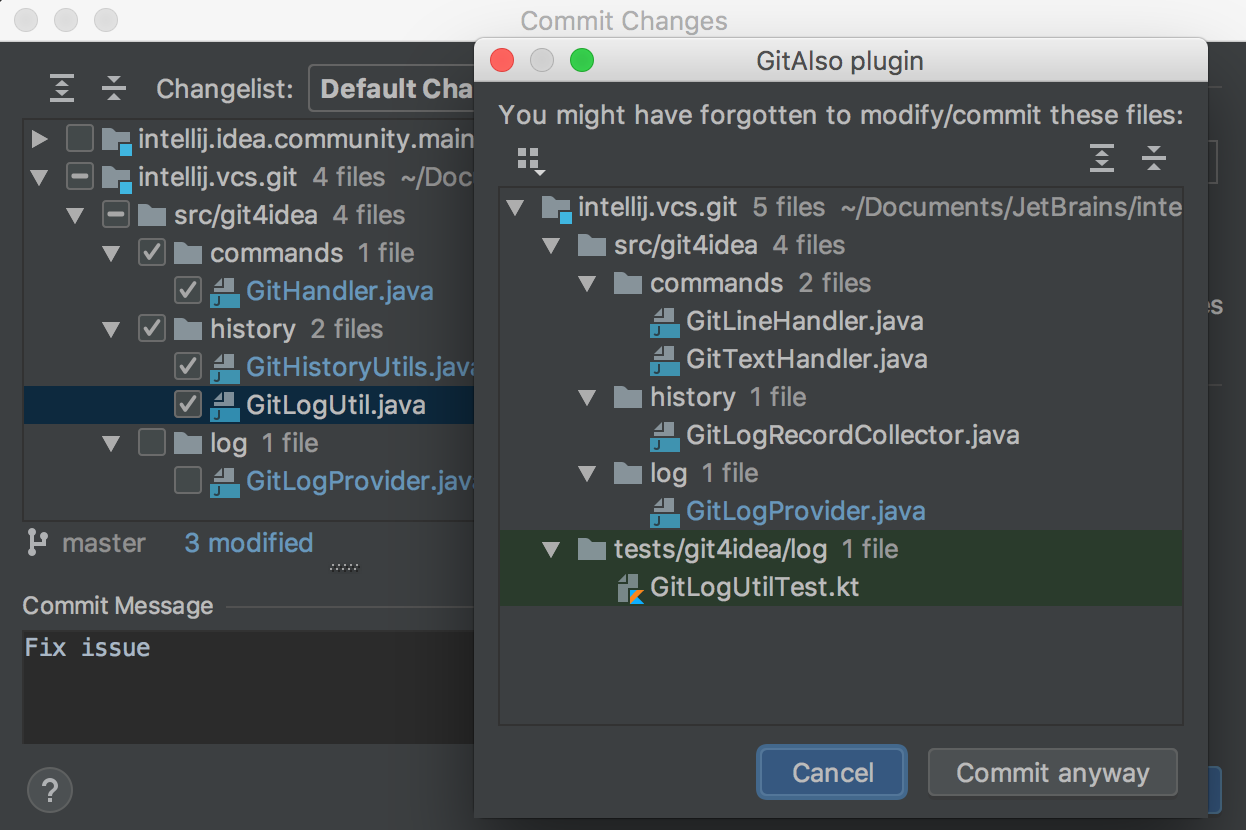
\includegraphics[scale=0.6]{GitAlso.png}
\end{figure}
Пользовательский интерфейс плагина должен показывать файлы, который пользователь возможно <<забыл>> изменить. Для показа таких файлов было решено открывать диалог с деревом файлов. Для показа дерева файлов использовалось готовое решение, которое называется $ChangesBrowser$. Пример показа рекомендации можно увидеть на рисунке  \ref{git-also-screen}.
\subsection{Персонализация решающей функции}
Для улучшения качества показываемых рекомендаций было принято решение использовать взаимодействие пользователя с плагином в целях изменения границы срабатывания решающей функции. На основе нажатий пользователем кнопок Commit Anyway и Cancel мы будем обновлять границу, используя метод $updateState$ приведенный в листинге \ref{personalization}, и сохранять ее в локальное состояние.
\section{Плагин ChangeReminder}
Исходя из результатов анализа статистики собранной в пункте \ref{jet-stat-logs} и анализа в пункте полученной статистики
 %TODO%
, а также отзывов внутри компании, стало понятно, что пользовательский интерфейс плагина GitAlso представленный в пункте \ref{git-also-ui} нужно изменить, избавившись от модальности. Тогда автором работы было принято решение переместить функциональность плагина GitAlso из коммит хука во вкладку Local Changes. В приведенной вкладке показаны файлы, который пользователь модифицировал, добавил, удалил из системы контроля версии. Представим, что пользователь будет сохранять в репозиторий все файлы, которые расположены в его списке изменений по умолчанию. Будем делать рекомендации для данных файлов при каждом их изменении и при изменении репозитория. В связи с такими изменениями было решено создать новый плагин и назвать его ChangeReminder. По большей части функциональность плагина основана на плагине GitAlso, но есть и существенные изменения в архитектуре.
\subsection{Архитектура}
\begin{figure}[!h]
\caption{Схема архитектуры плагина ChangeReminder}\label{ChangeReminder-arch}
\centering
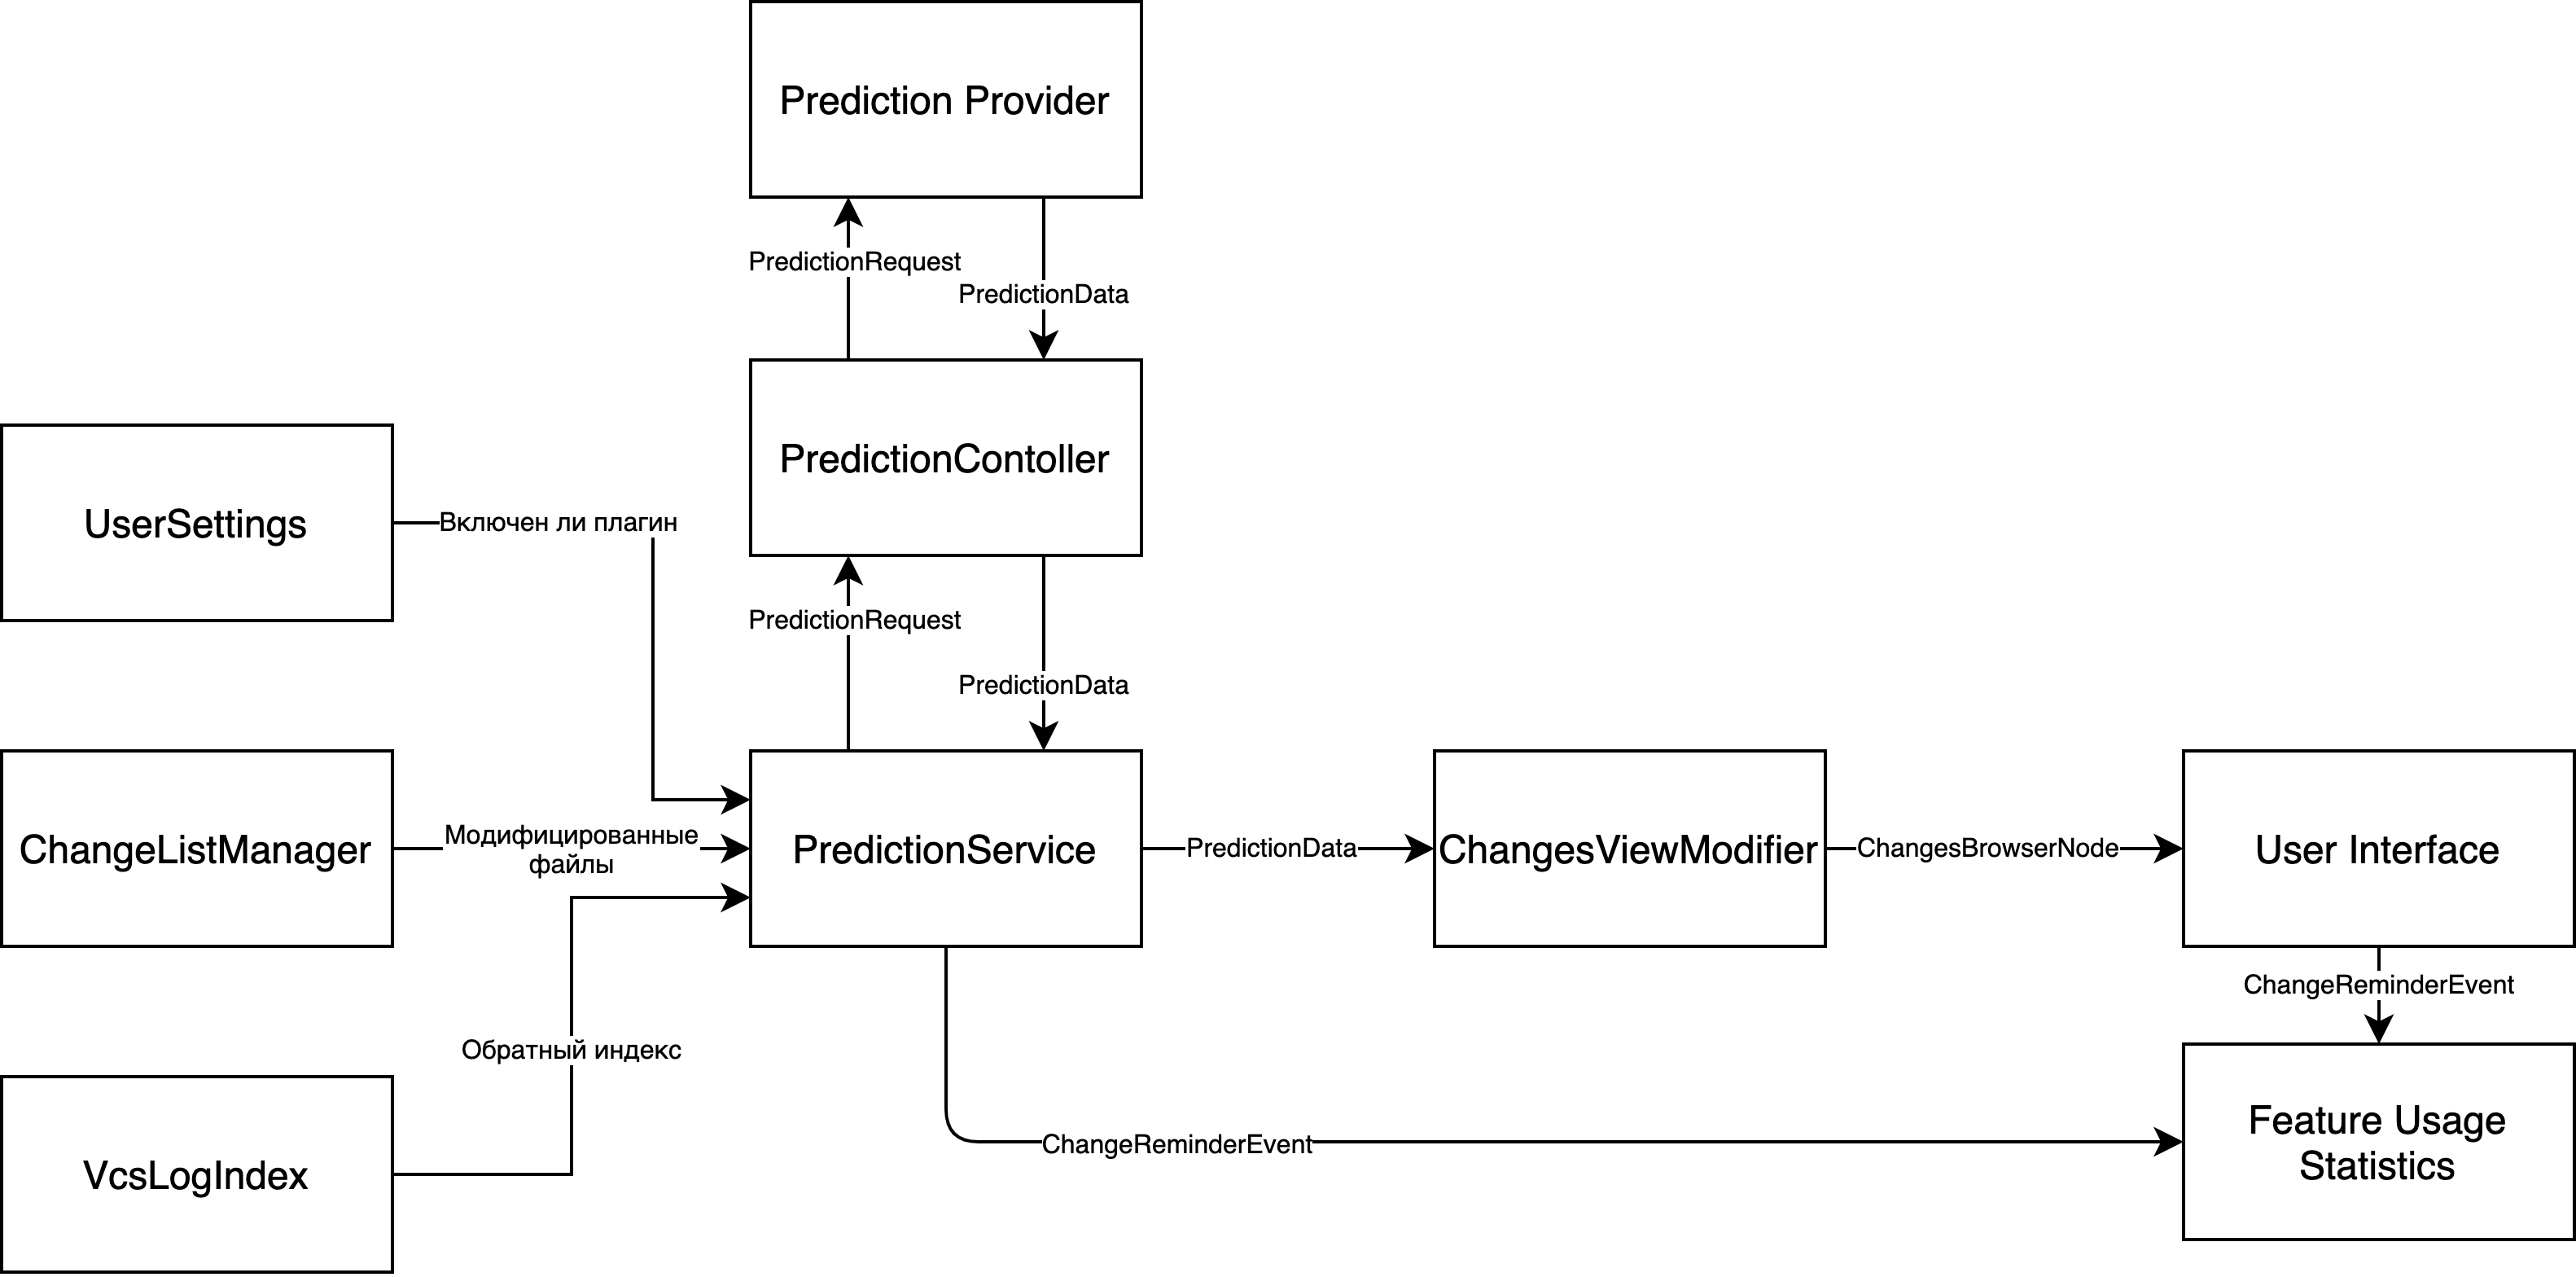
\includegraphics[scale=0.12]{ChangeReminderArch.png}
\end{figure}
Рекомендация файлов пользователю происходит по следующему алгоритму:
    \begin{itemize}[label={\textbullet}]
        \item Пользователь модифицирует файл/изменяется состояние одного из репозиториев.
        \item $ChangeListManager$ сообщает в $PredictionService$ о том, что список изменений по умолчанию изменился.
        \item $PredictionService$ запрашивает у $UserSettings$ включен ли плагин, если нет, то дальнейшие действия не происходят.
        \item $PredictionService$ запрашивает у $VcsLogIndex$ обратный индекс для текущих репозиториев, если индекс еще не готов, то дальнейшие действия не происходят.
        \item $PredictionService$ отправляет $PredictionRequest$ на обработку в $PredictionController$.
        \item $PredictionController$ занимается обработкой запроса и отдает $PredictionData$~-- результат работы в $PredictionService$
        \item $PredictionService$ запрашивает обновление у $ChangesViewModifier$
        \item $ChangesViewModifier$ из данной $PredictionData$ создает $ChangesBrowserNode$, которая рисуется в пользовательстком интерфейсе.
    \end{itemize}
$PredictionService$ и действия пользователя с интерфейсом записываются в сервисе Feature Usage Statistics (см. пункт \ref{fus-main}). Описанный выше алгоритм представлен на рисунке \ref{ChangeReminder-arch}. Рассмотрим каждую компоненту подробнее:\\
$UserSettings$~-- наследник $SimplePersistentStateComponent$, который используется для сохранения информации в локальное хранилище. В данном классе сохранено состояние $isPluginEnabled$, которое показывает, должен плагин делать рекомендации или нет. На изменения $UserSettings$ можно подписаться используя реализацию интерфейса $PluginStatusListener$.\\
$ChangeListManager$~-- менеджер, который хранит информацию о состоянии списков изменений, которые показываются во вкладке Local Changes. На изменения состояния менеджера можно подписаться используя реализацию интерфейса $ChangeListAdapter$\\
$VcsLogIndex$~-- класс, который подсчитывает и хранит обратный индекс для каждого репозитория. На окончание подсчета обратного индекса можно подписаться используя реализацию интерфейса $VcsLogIndex.IndexingFinishedListener$. На создание нового индекса или удаление старого можно подписаться используя реализацию интерфейса $VcsProjectLog.ProjectLogListener$\\
Важный момент, который стоит отметить~-- это то, что события от слушателей могут приходить из разных потоков, поэтому важно сделать сервис, который является потоко-безопасным.\\
$PredictionProvider$~-- класс разработанный в пункте TODO. Его главной задачей является предоставление рекомендации на основе данного коммита и истории репозитория.\\
$PredictionController$~-- имплементация интерфейса $SingleTaskController$. Главной задачей данного класса является контроль за выполнением подсчета рекомендации. Благодаря этому сервису подсчет осуществляется в одном потоке, притом при появлении нового запроса на подсчет, предыдущий прерывается, и выполняется новый в том же потоке.\\
$PredictionRequest$~-- класс, который умеет получать данные, нужные для работы ML модели. \\
$PredictionData$~-- класс, представляющий из себя алгебраический тип данных. Он может быть или $Prediction$ и содержать файлы рекомендованные моделью, или быть $EmptyPrediction$ и содержать причину, по которой предсказание не было подсчитано.
Всего есть несколько видов причин, почему предсказание могло быть не посчитано.\\
$ChangesViewModifier$~-- интерфейс разработанный автором работы. Он позволяет добавлять новые вершины с детьми в дерево представленное во вкладке Local Changes.\\
$PredictionService$~-- основной потоко-безопасный класс реализации ChangeReminder плагина. Его задачами является слушать изменения в сервисах указанных выше, отдавать новые данные в $PredictionController$ для дальнейшего подсчета рекомендации, получать результат в виде $PredictionData$, создавать запрос в Feature Usage Statistics на добавление статистики о данной рекомендации, и отдавать рекомендацию на отрисовку в $ChangesViewModifier$.
\subsection{Пользовательский интерфейс}
\begin{figure}[!h]
\caption{Пользовательский интерфейс плагина ChangeReminder}\label{ChangeReminder-ui}
\centering
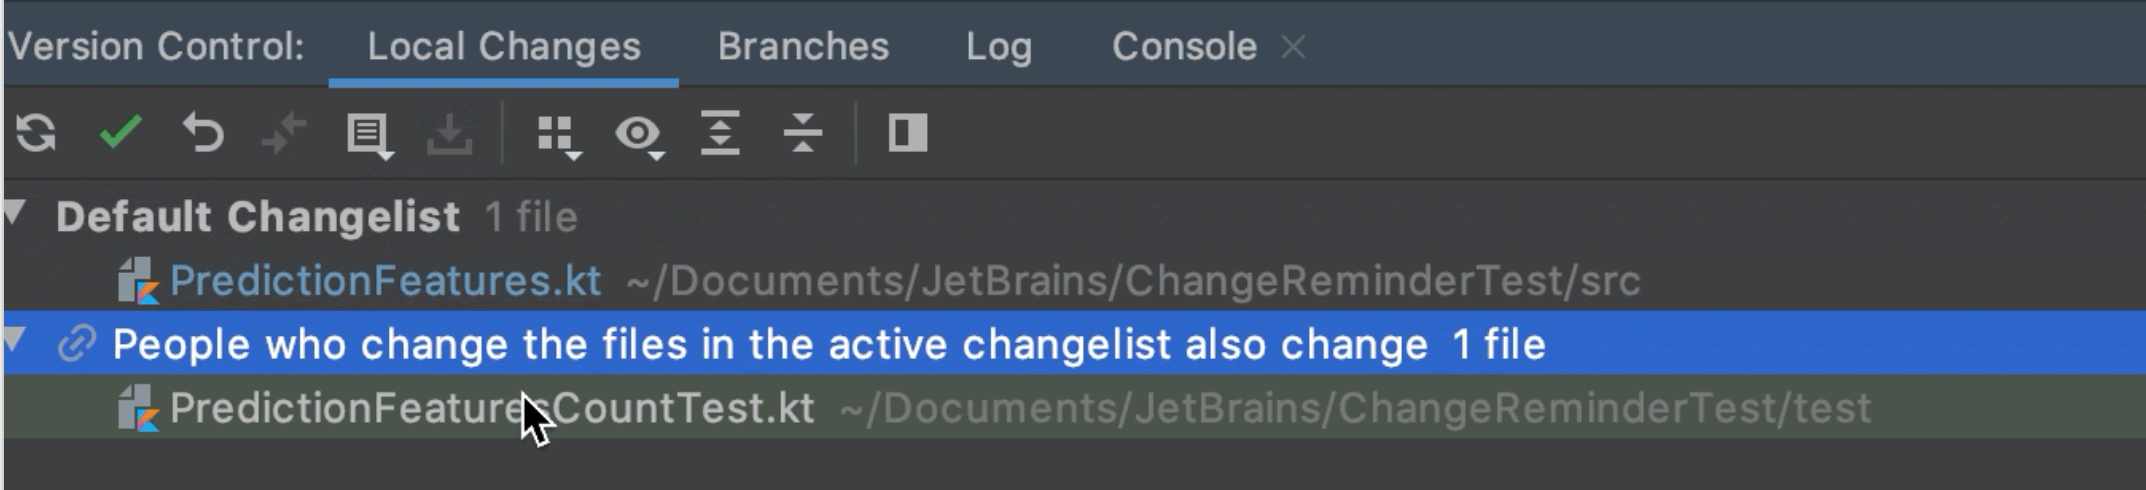
\includegraphics[scale=0.4]{ChangeReminderUI.png}
\end{figure}
Пользовательский интерфейс плагина ChangeReminder представляет из себя вершину в дереве изменений во вкладке Local Changes (см рисунок \ref{ChangeReminder-ui}). Вершина называется People who change the files in the active changelist also change. Если рекомендация составляет пустое множество файлов, то вершина становится невидимой.
\section{Практическое применение}
Плагин ChangeReminder идет в комплекте с продуктами на основе IntelliJ платформы, начиная с версии 2019.2.
\section{Планы на будущее}
TODO





%TODO
\section{Сбор статистики}\label{stats-main}
Для того, чтобы понимать, насколько хорошо работает наша решающая функция у пользователей в реальных условиях, а не на искусственно созданном наборе данных, было решено использовать сбор статистики. Также, с помощью пользовательских логов можно понять, что нужно изменить в нашей модели, чтобы число благоприятных исходов увеличилось. Для этого были записаны факторы для пар файлов, которые использовались для их для дальнейшего обучения. Не стоит забывать о том, что интерфейс плагина должен подходить пользователям. Используя статистику мы сможем понять реакцию пользователей на наши сообщения. Для этого был посчитан процент случаев, когда пользователь смотрел на предложенные файлы и когда проигнорировал нашу рекомендацию. Всего было сделано две реализации сбора пользовательской статистики. В начале статистика собиралась с использованием серверов JetStat, затем был совершен переход на более современный, встроенный в IntelliJ платформу сервис~-- Feature Usage Statistics (FUS).
\subsection{С использованием серверов JetStat}
Первая итерация сбора пользовательских логов использовала сервера внутреннего сервиса сбора и анализа статистики JetStat. Общение с JetStat серверами происходит по протоколу HTTP. Статистика пользователя для JetStat представляется в виде множества строк отчета, их формат будет изложен в секции \ref{report-line}. Отправлять пользовательские логи можно как в сжатом, так и в текстовом виде (для этого используются разные url).
\subsubsection{Модель пользовательских логов}
Пользовательские логи в JetStat представляют из себя конечный автомат. Состояние автомата~-- это данные описывающие состояние системы. А переход~-- это пользовательское действие.
\subsubsection{Строка отчета плагина}\label{report-line}
Каждая строка отчета, отправляемого в JetStat, представляет из себя части соединенные символом табуляции:
    \begin{itemize}[label={\textbullet}]
        \item $timestamp$ -- время, когда произошло пользовательское действие.
        \item $recorderId$ -- идентификатор отправителя статистики.
        \item $recoderVersion$ -- версия отправителя статистики.
        \item $userId$ -- идентификатор пользователя (создается при установке IDE).
        \item $sessionId$ -- идентификатор сессии (создается при открытии IDE).
        \item $bucket$ -- идентификатор группы (используется для A/B экспериментов).
        \item $actionType$ -- идентификатор действия пользователя.
        \item $actionJson$ -- информация о состоянии, в которое перешел пользователь.
    \end{itemize}

Рассмотрим конкретнее, какие типы действий пользователя отправлялись плагином:
    \begin{itemize}[label={\textbullet}]
        \item $COMMIT\_CLICKED$ -- нажатие кнопки Commit в Commit Dialog.
        \item $CANCEL$ -- нажатие кнопки Cancel
        \item $COMMIT$ -- нажатие кнопки Commit Anyway
    \end{itemize}

В информации о состоянии содержался $json$ в котором было несколько полей:
    \begin{itemize}[label={\textbullet}]
        \item $REPOSITORY$ -- уникальный для пользователя идентификатор репозитория.
        \item $FILES$ -- уникальные для репозитория идентификаторы файлов в коммите.
        \item $TIME$ -- время, затраченное на подсчет рекомендации.
        \item $PREDICTION$ -- уникальные для репозитория идентификаторы файлов, рекомендованные для модификации и добавления в коммит.
        \item $FACTORS$ -- факторы посчитанные для каждого рекомендованного файла.
    \end{itemize}
Идентификаторы репозитория, файлов и коммитов создает IntelliJ платформа. По данным идентификаторам нельзя идентифицировать пользователя. Таким образом, никакой приватной информации не отправляется. К тому же, при первом запуске IDE с плагином пользователю показывается нотификация о том, что плагин отправляет полностью анонимные данные для улучшения качества решающей функции.
\subsubsection{Реализация записи и отправки пользовательских логов}
\begin{figure}[!h]
\caption{Схема записи и отправки пользовательских логов}\label{jet-stat-logs}
\centering
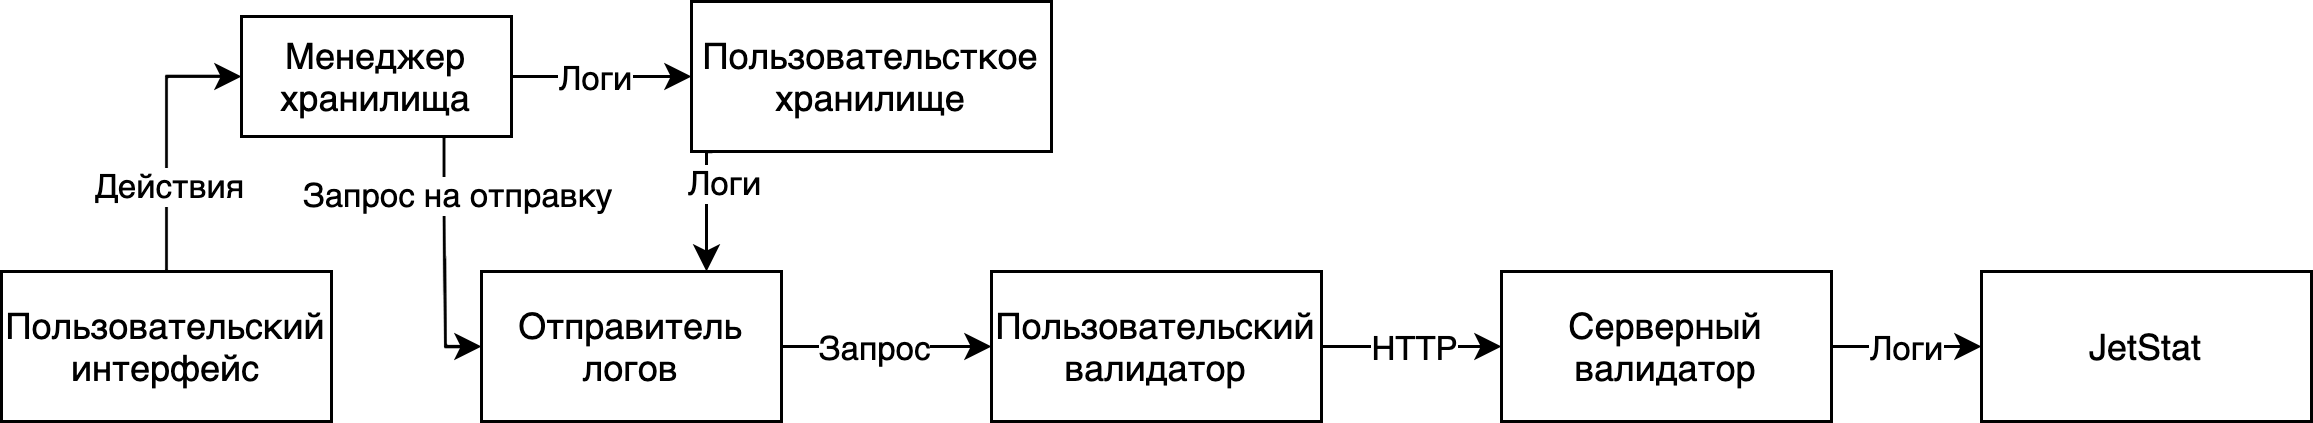
\includegraphics[scale=0.2]{JetStat.png}
\end{figure}
Реализация записи и отправки пользовательских логов показана на рисунке \ref{jet-stat-logs}. Принцип работы является достаточно популярным. При совершении пользователем какого-то действия над интерфейсом, это действие отправляется к менеджеру хранилища, который создает правильные строки отчета и сохраняет их в локальное хранилище. После этого менеджер хранилища отправляет запрос отправителю логов, чтобы сервис отправил накопившиеся данные на сервер. Если данных в локальном хранилище достаточно, то из них отправитель логов собирает HTTP запрос на сервер. Затем идет переход к одной из самых важных частей реализации~-- валидаторам. Перед тем, как отправлять данные на сервер, очень важно понять, не нарушена ли их консистентность (например, пользователю была показана рекомендация, но он ничего с ней не сделал). Для проверки консистентности данных был создан валидатор, который присутствует, как на стороне клиента, так и на стороне сервера. Только после того, как HTTP запрос прошел валидацию на клиентской стороне, он отправляется на сервер JetStat, где расположен серверный валидатор. Если пришедшие данные консистентны, то они сохраняются на сервер и ждут дальнейшей обработки.
\subsection{С использованием Feature Usage Statistics}\label{fus-main}
Следующая итерация сбора статистики плагина использовала сервис Feature Usage Statistics (FUS). FUS встроен в IntelliJ платформу.
\subsubsection{Модель пользовательских логов}
Пользовательские логи сервиса FUS представляют из себя набор событий системы. Часто, но не всегда, эти события порождаются действиями пользователя.
\subsubsection{Реализация отправки пользовательских логов}
Отправка пользовательских логов с помощью сервиса FUS является более простой, в сравнении с отправкой статистики на сервера JetStat. Feature Usage Statistics сам занимается хранением, валидацией и отправкой данных. Нашему приложению достаточно собрать $FeatureUsageData$ объект и передать его в FUS.
\printmainbibliography

\appendix

\chapter{Персонализация решающей функции}
\begin{lstlisting}[caption={Персонализация решающей функции},label={personalization}, language=Java, tabsize=2, basicstyle=\fontsize{10}{10}\selectfont\ttfamily]
private fun safeUpdateThreshold(newValue: Double) {
    val minThreshold = 0.0
    val maxThreshold = 1.0
    currentState.threshold = min(maxThreshold, max(minThreshold, newValue))
}

fun updateState(type: UserAction) {
    val gamma = 0.9
    val minimalStep = 0.05
    val chunksToBorderCount = 7


    if (type == UserAction.CANCEL && currentState.step <= 0) {
        safeUpdateThreshold(currentState.threshold - 0.005)
        currentState.lastAction = type
        return
    }
    currentState.lastAction = type

    currentState.step *= gamma
    currentState.step = when (type) {
        UserAction.COMMIT -> {
            min((1 - currentState.threshold) / chunksToBorderCount,
                    currentState.step + minimalStep)
        }
        UserAction.CANCEL -> {
            max(-currentState.threshold / chunksToBorderCount,
                    currentState.step - minimalStep)
        }
    }
    safeUpdateThreshold(currentState.threshold + currentState.step)
}
\end{lstlisting}
\end{document}